\documentclass[../../main.tex]{subfiles}
\begin{document}
\begin{oframed}
  \subfile{problem}
\end{oframed}

{\bf [解答]}

\begin{figure}[htb]
  \centering
  \begin{tikzpicture}[>=stealth, every node/.style={font=\small}]
    % 直方体の頂点座標
    % 底面
    \coordinate (A) at (0, 0);          % 手前左下
    \coordinate (B) at (2.6, 0);        % 手前右下
    \coordinate (Bp) at (3.8, 0.7);     % 奥右下
    \coordinate (Ap) at (1.2, 0.7);     % 奥左下 (隠れ頂点)

    % 上面
    \coordinate (D) at (0, 1.8);        % 手前左上
    \coordinate (C) at (2.6, 1.8);      % 手前右上 (代表頂点)
    \coordinate (Cp) at (3.8, 2.5);     % 奥右上
    \coordinate (Dp) at (1.2, 2.5);     % 奥左上

    % 上面のハッチング
    \fill[pattern=north east lines, pattern color=blue!35]
    (D) -- (C) -- (Cp) -- (Dp) -- cycle;

    % 奥の隠れ線 (破線)
    \draw[thick, dashed, gray!70!black] (Ap) -- (Bp);
    \draw[thick, dashed, gray!70!black] (Ap) -- (Dp);
    \draw[thick, dashed, gray!70!black] (A) -- (Ap);

    % 手前の稜線 (通常線)
    \draw[line width=1.1pt, gray!85!black] (A) -- (B);
    \draw[line width=1.1pt, gray!85!black] (A) -- (D);
    \draw[line width=1.1pt, gray!85!black] (D) -- (Dp) -- (Cp);
    \draw[line width=1.1pt, gray!85!black] (B) -- (Bp) -- (Cp);

    % 1つの頂点 C から出る3辺 (太線強調)
    \draw[line width=1.4pt, blue!85!black] (C) -- (D) node[midway, below] {$x$};
    \draw[line width=1.4pt, blue!85!black] (C) -- (Cp) node[midway, below right=-1pt] {$y$};
    \draw[line width=1.4pt, blue!85!black] (C) -- (B) node[midway, right=1pt] {$z$};

    % 基準となる頂点 C
    \node[circle, fill=red!85!black, inner sep=1.4pt] at (C) {};
  \end{tikzpicture}
  \caption{1つの頂点から出る3辺の長さが $x, y, z$ である直方体}
  \label{fig:cuboid_xyz}
\end{figure}

まず題意から
\begin{align}
  x,y,z>0 \label{eq:1} \\
  x+y+z=6  \label{eq:2}\\
  yz+zx+xy=9  \label{eq:3}
\end{align}
となる．

\subparagraph{(1)}

まず$s=y+z$，$t=yz$として，$y$，$z$の存在条件を考える．
\cref{eq:2,eq:3}から
\begin{align}
  \begin{cases}
    s=6-x \\
    t=x^2-6x+9
  \end{cases}\label{eq:4}
\end{align}
となる．

さて，\cref{eq:1,eq:4}から$y, z$は$p$の$2$次方程式
\begin{align}
  &p^2-sp+t=0\\
  \Longleftrightarrow &p^2-(6-x)p+(x^2-6x+9)=0
\end{align}
の正の$2$実解であるから，判別式$D$として
\begin{align}
  &
  \begin{cases}
    D\ge0  \\
    s,t>0
  \end{cases} \\
  \Longleftrightarrow
  &
  \begin{cases}\\
    (6-x)^2-4(x^2-6x+9)\ge0  \\
    6-x>0  \\
    x^2-6x+9>0
  \end{cases} \\
  \Longleftrightarrow
  &
  \begin{cases}\\
    (6-x)^2-4(x^2-6x+9)\ge0  \\
    6-x>0  \\
    x^2-6x+9>0
  \end{cases} \\
  \Longleftrightarrow
  &
  \begin{cases}
    0\le x\le 4  \\
    x<6  \\
    x \neq 3
  \end{cases} \\
  \Longleftrightarrow
  &   0\le x<3,3<x\le 4
\end{align}
となる．\cref{eq:1}と合わせて求める範囲は
\begin{align}
  0< x<3,3<x\le 4 \tag{(答)}
\end{align}
である．

\subparagraph{(2)}
$a=x+y+z$，$b=yz+zx+xy$，$c=xyz$とおく．すると$x$，$y$，$z$は$p$の$3$次方程式
\begin{align}
  &p^3-ap^2+bp-c=0  \nonumber\\
  \Longleftrightarrow&p^3-6p^2+9p-c=0 \label{eq:5}
\end{align}
の正の実数解である．故に\cref{eq:5}が正の$3$実解(重解含む)をもつ条件を求める．
このような条件は
\begin{align}
  y=f(p)=p^3-6p^2+9p
\end{align}
と$y=c$が$0<p$に$3$つの共有点(重解含む)を持つことである．
そこで$f(p)$の挙動を調べる．一階微分は
\begin{align}
  f'(p)&=3p^2-12p+9  \\
  &=3(p-1)(p-3)
\end{align}
であるから増減表は以下のようになる．

\begin{table}[htb]
  \centering
  \caption{$f(p)$ の増減表}
  \label{tab:fp_increments}
  \begin{tabular}{|c|c|c|c|c|c|}
    \hline
    $p$ & $\cdots$ & $1$ & $\cdots$ & $3$ & $\cdots$ \\ \hline
    $f'(p)$ & $+$ & $0$ & $-$ & $0$ & $+$ \\ \hline
    $f(p)$ & $\nearrow$ & $4$ & $\searrow$ & $0$ & $\nearrow$ \\ \hline
  \end{tabular}
\end{table}

従って，$y=f(p)$のグラフは下のようになり，故に$c$の値域は$0< c <3, 3< c \le4$である．

\begin{figure}[htb]
  \centering
  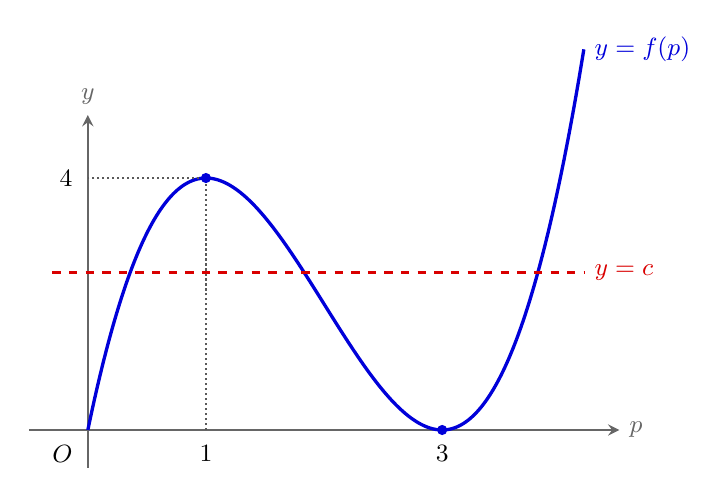
\begin{tikzpicture}[x=1.5cm, y=0.8cm, >=stealth, every node/.style={font=\small}]
    \draw[->, thick, gray!80!black] (-0.5, 0) -- (4.5, 0) node[right] {$p$};
    \draw[->, thick, gray!80!black] (0, -0.6) -- (0, 5.0) node[above] {$y$};
    \node[below left=2pt] at (0, 0) {$O$};

    % 曲線 y = p^3 - 6p^2 + 9p
    \draw[line width=1.2pt, blue!85!black, domain=0:4.2, samples=100, smooth]
    plot (\x, {(\x)^3 - 6*(\x)^2 + 9*(\x)}) node[right] {$y=f(p)$};

    % 極大点 (1, 4)
    \draw[densely dotted, thick, gray!70!black] (1, 0) -- (1, 4) -- (0, 4);
    \node[circle, fill=blue!85!black, inner sep=1.3pt] at (1, 4) {};
    \node[below=2pt] at (1, 0) {$1$};
    \node[left=2pt] at (0, 4) {$4$};

    % 極小点 (3, 0)
    \node[circle, fill=blue!85!black, inner sep=1.3pt] at (3, 0) {};
    \node[below=2pt] at (3, 0) {$3$};

    % 直線 y = c
    \draw[line width=1.0pt, red!85!black, dashed] (-0.3, 2.5) -- (4.2, 2.5)
    node[right] {$y=c$};
  \end{tikzpicture}
  \caption{$y=f(p)$ のグラフと直線 $y=c$}
  \label{fig:cubic_poly}
\end{figure}
さて，直方体の体積は$c$に等しいから$\max c=4\cdots$(答)である．

{\bf [別解]}

\subparagraph{(1)}

(2)の[解答]と同様に，$x, y, z$は$p$の$3$次方程式$p^3-6p^2+9p-c=0$の正の$3$実解であるから，$y=f(p)$と$y=c$の共有点の$p$座標である．ゆえにグラフから$x$の値域は$0<x<3, 3<x \le4$である．$\cdots$(答)
\newpage
\end{document}
